\documentclass[a4paper,12pt]{article} % Tipo de documento y tamaño de letra.
\usepackage[utf8]{inputenc} % Para que reconozca caracteres especiales como tildes.
\usepackage[spanish, es-nodecimaldot]{babel} % Para definir el idioma y el formato de fechas en español.
\usepackage{amsmath, amssymb} % Paquetes para símbolos y ecuaciones avanzadas (Para hacer una ecuación con un recuadro).
\usepackage{ragged2e} % Para justificar textos.
\usepackage{multicol} % Para crear columnas.
\usepackage{slashed} % Para generar números o variables canceladas (Una línea diagonal sobre el número o variable).
\usepackage{graphicx} % Paquete para poner graficas.
\usepackage{float} % Para poder dejar la imagen en un punto fijo del documento.
\usepackage{longtable} % Para tablas largas.
\usepackage{cancel} % Para hacer cancelaciones en medio de operaciones.
\usepackage{xcolor} % Para el color y esas cosas.
\usepackage{apacite} % Paquete para citas APA.
\usepackage{fancyhdr} % Para personalizar encabezados y pies de página.
\usepackage{geometry} % Para ajustar márgenes.
\usepackage{setspace} % Para ajustar el interlineado.
\usepackage{natbib} % Para manejar las citas y que no queden pegadas y feas :P.
\usepackage{hyperref} % Para que los enlaces funcionen con su URL.
\usepackage[version=4]{mhchem}  % Versión recomendada para mayor funcionalidad.
\usepackage{chemfig} %También para hacer estructuras químicas.
\usepackage{array} % Para mejor control de las columnas.
\usepackage{siunitx} % Para unidades físicas.


\pagestyle{fancy}
\fancyhf{} % Limpia encabezados y pies de página predeterminados
\fancyhead[L]{\textbf{BOLETÍN DE PROBLEMAS.}} % Encabezado izquierdo
\fancyhead[R]{\textbf{TERMODINÁMICA.}} % Encabezado derecho
\fancyfoot[C]{\thepage} % Número de página en el centro del pie

\geometry{headheight=12.96115pt, top=1in, bottom=1in, left=1in, right=1in}
\begin{document}


\begin{figure}[H]
	\centering
	
\includegraphics[width=0.5\textwidth]{Unir.jpg}
\end{figure}

\vspace{\baselineskip}

% Ajustamos manualmente todo ;)
\begin{center}
	\textbf{\Large } \\[0.9cm]
	\vspace{\baselineskip}
	\textbf{Liz Ángel Núñez Torres.} \\[0.6cm]
	\textbf{Grado en Física.} \\[0.6cm]
	\textbf{Universidad Internacional de La Rioja.} \\[0.6cm]
	\textbf{20 de Diciembre 2025.}
\end{center}


\newpage
\tableofcontents

\newpage

\begin{abstract}
\end{abstract}

\begin{justify}
	Para este documento, dirigido a la lectora \textbf{Valentina Zambrano} se ha puesto dos formatos para resultados.
\end{justify}



\begin{itemize}
	\item Para los resultados definitivos el color \textcolor{purple}{púrpura}.
	\item Para los resultado parciales el color \textcolor{brown}{marrón}.
\end{itemize}

\vspace{\baselineskip}

\section{Derivada de una Función.}

\begin{justify}
	Calcular la derivada de la función.
\end{justify}

\[ f\left( x \right) = x^2 \, e^{-2x} + \ln \left( 2x + 1 \right) \]

\begin{justify}
	Derivamos por separado cada término.
\end{justify}

\begin{multicols}{2}
	\begin{itemize}
		\item \( x^2 e^{-2x}. \)
	\end{itemize}

	\begin{itemize}
		\item \( \ln(2x + 1). \)
	\end{itemize}
\end{multicols}

\subsection{Regla del producto.}

\begin{justify}
	Para el primer término, usaremos la \textbf{regla del producto} para obtener su derivada.
\end{justify}

\[ \frac{d}{dx}\left[ x^2 e^{-2x} \right] = 2x \cdot e^{-2s} + x^2 \cdot \left( -2 e^{-2x}.  \right) \]

\[ 2xe^{-2x} - 2x^2 e^{-2x}. \]

\[ \textcolor{brown}{\boxed{2xe^{-2x} \left( 1 - x \right).}} \]

\subsection{Derivada del segundo término.}

\begin{justify}
	Ahora, desarrollaremos la derivada de \( \ln(2x + 1) \).
\end{justify}

\[ \frac{d}{dx}\left[ \ln(2x + 1) \right] = \frac{1}{2x +1 } \cdot 2. \]

\[ \textcolor{brown}{\boxed{\frac{2}{2x + 1}.}} \]

\subsection{Resultado.}

\begin{justify}
	Con los resultados previos, el resultado de la función será:
\end{justify}

\[ \textcolor{purple}{\boxed{ f'\left( x \right) = 2x e^{-2x} \left( 1 - x \right) + \frac{2}{2x + 1}. }} \]

\section{Diferencial de una Función.}

\begin{justify}
	Calcular la diferencial de la función de dos variables.
\end{justify}

\[ f \left( x , y \right) = x^2y + e^{-xy}. \]

\begin{justify}
	Como sabemos que la diferencial total de nuestra función es:
\end{justify}

\[ df = \frac{\partial f}{\partial x}dx + \frac{\partial f}{\partial y}dy \]

\begin{justify}
	Por lo tanto, haremos primero la derivada parcial respecto de \( \mathbf{x}\), luego respecto de \( \mathbf{y}\).
\end{justify}

\subsection{Derivada parcial respecto de \( x \).}

\[ \frac{\partial f}{\partial x} = \frac{\partial}{\partial x} \left( x^2 y \right) + \frac{\partial}{\partial x} \left( e^{-x} y^2 \right). \]

\[ \frac{\partial}{\partial x} \left( x^2 y\right) = 2xy. \]

\[ \frac{\partial}{\partial x} \left( e^{-x} y^2 \right) = \left( -1 \right) e^{-x} y^2. \]

\vspace{\baselineskip}

\[ \textcolor{brown}{\boxed{ \frac{\partial f}{\partial x} = 2xy - e^{-x}y^2. }} \]


\subsection{Derivada parcial respecto de \( y \).}

\[ \frac{\partial f}{\partial y} = \frac{\partial}{\partial y} \left( x^2 y \right) + \frac{\partial}{\partial y} \left( e^{-x} y^2 \right). \]

\[ \frac{\partial}{\partial y} \left( x^2 y \right) = x^2 \]

\[ \frac{\partial}{\partial y} \left( e^{-x} y^2 \right) = 2 e^{-x}y.  \]

\vspace{\baselineskip}

\[ \textcolor{brown}{\boxed{ \frac{\partial f}{\partial y} = x^2 + 2 e^{-x}y. }} \]


\subsection{ Diferencial de la función. }

\begin{justify}
	Como la diferencial total es:
\end{justify}

\[ df = \frac{\partial f}{\partial x}dx + \frac{\partial f}{\partial y}dy .\]

\begin{justify}
	Por lo tanto el resultado final es:
\end{justify}

\[ \textcolor{purple}{\boxed{ df = \left( 2xy - e^{-x} y^2 \right) dx + \left( x^2 + 2 e^{-x} y \right) dy . }} \]

\section{Expansión Isóbara.}

\begin{justify}
	Calcular el trabajo realizado en un sistema químico durante una expansión isóbara a una atmósfera de presión si el gas ocupa inicialmente el volumen \(22,4 \mathrm{l}\) y duplica su volumen.
\end{justify}

\begin{justify}
	\textbf{DATOS:}
\end{justify}

\begin{itemize}
	\item \( \mathrm{P} = 1 \, \mathrm{atm} \Rightarrow 1.013 \times 10^5 \, \mathrm{Pa}. \)
	\item \( V_1 = 22.4 \mathrm{L} \Rightarrow 2.24 \times 10^{-2} \, m^3 .\)
	\item \( V_2 = 2 \cdot V_1 \Rightarrow 44.8 \, \mathrm{L} \Rightarrow 4.48 \times 10^{-2}\, m^3. \)
\end{itemize}

\begin{justify}
	Para obtener el resultado, primero debemos recordar que en un proceso isobárico \textbf{la presión es constante}, además que la formula para este proceso es:
\end{justify}

\[ W = P \triangle V. \]

\begin{justify}
	Donde \( \triangle V \) es:
\end{justify}

\[ \triangle V = V_2 -  V_1 \]

\[ \triangle V = 4.48 \times 10^{-2} \, m^3 - 2.24 \times 10^{-2} \, m^3. \]

\[ \textcolor{brown}{\boxed{ \triangle V = 2.24 \times 10^{-2} \, m^3.}} \]

\subsection{Trabajo.}

\begin{justify}
	Por lo tanto el trabajo será:
\end{justify}

\[ W = 1.013 \times 10^5 \, \mathrm{Pa} \cdot 2.24 \times 10^{-2} \, m^3 \]

\vspace{\baselineskip}

\[ \textcolor{purple}{\boxed{ W = 2270 \, J. }} \]

\begin{justify}
	Podemos argüir que el \textbf{sistema realiza trabajo} por esto es positivo.
\end{justify}

\section{Proceso Adiabático.}

\begin{justify}
	Calcular el aumento de temperatura de \( 1 \, \mathrm{L} \) de agua si su calor específico es constante y de \(1calg^{-1}  \SI{}{\degreeCelsius}^{-1}  \) y se realiza un trabajo adiabático de \( 5 \mathrm{J}\).
\end{justify}

\begin{justify}
	\textbf{DATOS:}
\end{justify}

\begin{multicols}{2}
	\begin{itemize}
		\item \( V = 1\,\mathrm{L} \Rightarrow 1 \, \mathrm{kg}. \)
		\item \( c = 4184 \, \mathrm{J}/ \mathrm{kg} \cdot \SI{}{\degreeCelsius}. \)
		\item \( W = 5 \, \mathrm{J}. \)
	\end{itemize}
\end{multicols}

\begin{justify}
	Sabemos que en un proceso adiabático no hay tranferencia de calor hacia o desde el sistema.\textbf{ Todo el cambio de energía interna se debe al trabajo realizado}, en nuestro caso el trabajo se hace sobre el sistema, el agua, porque es positivo. 
\end{justify}


\subsection{Primera Ley.}

\begin{justify}
	Usamos la \textbf{primera Ley de la Termodinámica} que es:
\end{justify}

\[ \triangle U = Q + W \]

\begin{justify}
	Siendo \( Q = 0 \)  tendremos entonces:
\end{justify}

\[ \textcolor{brown}{\boxed{ \triangle U = W.}} \]

\begin{justify}
	Para un líquido, la variación de energía interna se debe principalmente al cambio de temperatura.
\end{justify}

\[ \textcolor{brown}{\boxed{ \triangle U = mc \triangle T.}} \]

\begin{justify}
	Por lo tanto, igualamos y despejamos la variación de energía interna.
\end{justify}

\[ W = mc \triangle T. \]

\[ \triangle T = \frac{W}{mc}. \]

\subsection{Aumento de Temperatura.}

\begin{justify}
	Por lo tanto el aumento de temperatura es:
\end{justify}

\[ \triangle T = \frac{5 \, \cancel{\mathrm{J}}}{ 1 \cancel{\mathrm{kg}} \cdot 4184 \cancel{\mathrm{J}} / \cancel{\mathrm{kg}} \SI{}{\degreeCelsius}}. \]

\vspace{\baselineskip}

\[\textcolor{purple}{\boxed{ \triangle T = 1.195 \times 10^{-3} \, \SI{}{\degreeCelsius}. }}\]

\begin{justify}
	El aumento de temperatura es pequeño porque el trabajo realizado fue bajo.
\end{justify}

\section{Expansión Isotérmica.}

\begin{justify}
	Calcular el trabajo realizado por la expansión de dos moles de un gas ideal en una expansión isoterma \((T = \SI{42}{\degreeCelsius})\) en la que la presión se reduce a la mitad.
\end{justify}

\begin{justify}
	\textbf{DATOS:}
\end{justify}

\begin{itemize}
	\item \( T \, \SI{42}{\degreeCelsius} \Rightarrow 315.15 \, \mathrm{K}. \)
	\item \( \mathrm{n} = 2 \, \mathrm{mol}. \)
	\item \( R = 8.314 \, \mathrm{J}/ \mathrm{mol} \, \mathrm{k}. \)
\end{itemize}

\begin{justify}
	Sabemos que los procesos isotérmicos la temperatura es constante y la expansión es reversible \( W > 0\).
\end{justify}

\begin{justify}
	Usaremos entonces:
\end{justify}

\[ W = nRT \ln\left(\frac{V_2}{V_1}\right). \]

\begin{justify}
	Como es Isoterma y la presión se reduce a la mitad.
\end{justify}

\[ P_1 \, V_1 = P_2 \, V_2 \Rightarrow \frac{V_2}{V_1} = \frac{P_1}{P_2} \]

\[ \textcolor{brown}{\boxed{\frac{P_1}{P_2} = 2. }} \]

\subsection{Trabajo por la Expansión.}

\[ W = 2 \cancel{\mathrm{mol}} \cdot 8.314 \, \mathrm{J}/ \cancel{\mathrm{mol}} \, \cancel{\mathrm{K}} \cdot 315.15 \, \cancel{K} \, \ln(2). \]

\[ W = 5.237 \, \mathrm{J}  \cdot 0.693. \]

\[ \textcolor{purple}{\boxed{ W = 3630 \, \mathrm{J}. }} \]

\section{Proceso Termodinámico Cíclico.}

\begin{justify}
	En un proceso termodinámico cíclico donde en la primera etapa se absorbe un calor equivalente a \( 4,56 \, \mathrm{cal} \) y se realiza un trabajo sobre el sistema de \(3 \mathrm{J} \), calcular el calor absorbido en la segunda etapa si el sistema realiza sobre los alrededores un trabajo de \( 2,1 \, \mathrm{J} \).
\end{justify}

\begin{justify}
	\textbf{DATOS:}
\end{justify}

\begin{itemize}
	\item \( Q = 4,56 \, \mathrm{cal} \Rightarrow 19.08 \, \mathrm{J}. \)
	\item \( W_1 = 3 \, \mathrm{J}. \)
	\item \( W_2 = 2.1 \mathrm{J}. \)
\end{itemize}

\begin{justify}
	\textbf{Primera Ley.}
\end{justify}

\[ \triangle U_{ciclo} = 0 .\]

\begin{justify}
	En un ciclo.
\end{justify}

\[ \Sigma Q + \Sigma W = 0. \]

\subsection{Etapa 1.}

\begin{justify}
	Sabemos que:
\end{justify}

\begin{itemize}
	\item Calor absorbido.
	\item Trabajo sobre sistema.
\end{itemize}

\[ W = -3 \, \mathrm{J}. \]

\begin{justify}
	Cambio de energía interna.
\end{justify}

\[ \triangle U_1 = Q_1 - W_1. \]

\[ \triangle U_1 = 19.08 \, \mathrm{J} - \left( -3 \right). \]

\[ \textcolor{brown}{\boxed{ \triangle U_1 = 22.08 \, \mathrm{J}.}} \]

\subsection{Etapa 2.}

\begin{justify}
	El sistema realiza trabajo a los alrededores.
\end{justify}

\[ W_2 = 2.1 \, \mathrm{J}. \]

\begin{justify}
	Por lo tanto.
\end{justify}

\[ \triangle U_2 = Q_2 - 2.1 \mathrm{J}. \]

\begin{justify}
	Como es un proceso cíclico.
\end{justify}

\[ \triangle U_1 + \triangle U_2 = 0. \]

\[ 22.8 \mathrm{J} + \left( Q_2 -  2.1 \, \mathrm{J} \right) = 0. \]

\[ Q_2 = 2.1 \, \mathrm{J} - 22.8 \mathrm{J}. \]

\[ \textcolor{purple}{\boxed{ Q_2 = - 19.98 \, \mathrm{J} }} \]

\section{Proceso Isostérico.}

\begin{justify}
	Calcular la variación de energía interna en un proceso isostérico en el que se absorben \( 45,4 \, \mathrm{cal}\).
\end{justify}

\begin{justify}
	\textbf{DATOS:}
\end{justify}

\begin{itemize}
	\item \( W = 0 \)
	\item \( Q = 45.4 \, \mathrm{cal}  \Rightarrow 185.76 \, \mathrm{J}. \)
\end{itemize}

\subsection{Primera Ley.}

\begin{justify}
	\textbf{Aplicamos la primera Ley de la termodinámica.}
\end{justify}

\[ \triangle U = Q - W. \]

\begin{justify}
	Como es Isostérica, el volumen es constante, por esto, el trabajo realizado es \textbf{cero}.
\end{justify}

\[ \triangle U = Q - 0. \]

\[ \triangle U = 185.76 \, \mathrm{J} - 0. \]

\[ \textcolor{purple}{\boxed{\triangle U = 185.76 \, \mathrm{J} .}} \]

\section{Proceso Isotermo.}

\begin{justify}
	En un proceso isotermo a \( \SI{25}{\degreeCelsius} \) un gas ideal, que ocupa inicialmente un volumen de \( 24 \, \mathrm{L}\), aumenta su presión de \(1 \, \mathrm{atm}\) a \(3,5 \, \mathrm{atm}\). Calcular el volumen final que ocupará el gas.
\end{justify}

\begin{justify}
	\textbf{DATOS:}
\end{justify}

\begin{itemize}
	\item \( T = \SI{25}{\degreeCelsius} \Rightarrow 298 \, \mathrm{K}.  \)
	\item \( V_1 = 24 \, \mathrm{L}  \Rightarrow 24 \times 10^{-3} \, \mathrm{m}^3. \)
	\item \( P_1 = 1 \, \mathrm{atm}  \Rightarrow 101325 \, \mathrm{Pa}. \)
	\item \( P_2 = 3.5  \, \mathrm{atm} \Rightarrow 354637.5 \, \mathrm{Pa}. \)
\end{itemize}

\subsection{Ley de Boyle - Mariotte.}

\[ P_1 V_1 = P_2 V_2. \]

\begin{justify}
	Despejamos el volumen final \( \mathbf{V_2} \).
\end{justify}

\[ V_2 = \frac{P_1 V_2}{P_2}. \]

\vspace{\baselineskip}

\[ V_2 = \frac{101325 \, \cancel{\mathrm{Pa}} \cdot 24 \times 10^{-3} \, \mathrm{m}^3.}{ 354637.5 \, \cancel{\mathrm{Pa}} } \]

\vspace{\baselineskip}

\[ \textcolor{purple}{\boxed{ V_2 = 6.85 \times 10^{-3} \, \mathrm{m}^3 .}} \]

\section{Transformación Isobárica.}

\begin{justify}
	En una transformación isobárica, la temperatura de un gas asciende de \( \SI{25}{\degreeCelsius} \) a \( \SI{100}{\degreeCelsius} \). Calcular el volumen final del gas si inicialmente su volumen era \( 4 \, \mathrm{L} \).
\end{justify}

\begin{justify}
	\textbf{DATOS:}
\end{justify}

\begin{itemize}
	\item \( T_1 = \SI{25}{\degreeCelsius}  \Rightarrow 298 \, \mathrm{K}. \)
	\item \( T_2 = \SI{100}{\degreeCelsius}  \Rightarrow 373 \, \mathrm{K}. \)
	\item \( V_1 = 4 \, \mathrm{L} \Rightarrow 4 \times 10^{-3} \, \mathrm{m}^3. \)
\end{itemize}

\begin{justify}
	Como la presión es constante (proceso isobárico) para un gas ideal.
\end{justify}

\subsection{Ley Charles.}

\[ \frac{V}{T}. \]

\begin{justify}
	Despejamos y sustituimos.
\end{justify}

\[ \frac{V_1}{T_1} = \frac{V_2}{T_2}. \Rightarrow V_2 = \frac{V_1 \cdot T_2}{T_1} \]

\vspace{\baselineskip}

\[ V_2 = \frac{4 \times 10^{-3} \, \mathrm{m}^3 \cdot 373 \, \cancel{\mathrm{K}} }{298 \, \cancel{\mathrm{K}}} \]

\vspace{\baselineskip}

\[ \textcolor{purple}{\boxed{V_2 = 5 \times 10^{-3} \, \mathrm{m}^3 .}} \]

\section{Volumen de un Mol.}

\begin{justify}
	Calcular el volumen que ocupa un mol de un gas ideal a la presión atmosférica y a la temperatura ambiente de \( \SI{25}{\degreeCelsius} \).
\end{justify}

\begin{justify}
	\textbf{DATOS:}
\end{justify}

\begin{itemize}
	\item \( T_1 = \SI{25}{\degreeCelsius} \Rightarrow 298 \, \mathrm{K}. \)
	\item \( P = 1 \, \mathrm{atm} \Rightarrow 101325 \, \mathrm{Pa}. \)
	\item \( n = 1 \, \mathrm{mol}. \)
\end{itemize}

\begin{justify}
	Cómo tenemos un gas ideal a presión atmosférica, usaremos la ley de los gases ideales para su solución.
\end{justify}

\subsection{Ley de los Gases Ideales.}

\[ PV = nRT. \]

\[ V = \frac{nRT}{P} \]

\begin{justify}
	Sustituimos.
\end{justify}

\[ V = \frac{1 \, \cancel{\mathrm{mol}} \cdot 8.314 \, J/ \cancel{\mathrm{mol}} \, \cancel{\mathrm{K}} \cdot 293 \, \cancel{\mathrm{K}}}{101325 \, \mathrm{Pa}}. \]

\vspace{\baselineskip}

\[ \textcolor{purple}{\boxed{ V = 2,40 \times 10^{-2} \, \mathrm{m}^3. }} \]

\section{Expansión Isotérmica.}

\begin{justify}
	Calcular la variación de energía interna de un gas ideal que se expande isotérmicamente a \( \SI{20}{\degreeCelsius} \), de un volumen inicial de \( 2 \, \mathrm{L} \) a \( 3,5 \, \mathrm{L} \). Calcular el calor absorbido (en calorías) sabiendo que la presión inicial es de \( 1 \, \mathrm{atm} \).
\end{justify}

\begin{justify}
	\textbf{DATOS:}
\end{justify}

\begin{multicols}{2}
	\begin{itemize}
		\item \( T = \SI{20}{\degreeCelsius} \Rightarrow 293,15 \, \mathrm{K}. \)
		\item \( V_1 = 2 \, \mathrm{L} \Rightarrow 2 \times 10^{-3} \, \mathrm{m}^3. \)
		\item \( V_2 = 3.5 \, \mathrm{L} \Rightarrow 3.5 \times 10^{-3} \, \mathrm{m}^3. \)
		\item \( P_1 = 1 \, \mathrm{atm} \Rightarrow 101325 \, \mathrm{Pa}. \) 
	\end{itemize}
\end{multicols}

\begin{justify}
	Para un gas ideal isotermo la variación de energía interna es:
\end{justify}

\[ \textcolor{brown}{\boxed{ \triangle U = 0. }} \]

\subsection{Ley de los Gases Ideales.}

\begin{justify}
	Como es un gas ideal, usaremos la formula de los gases ideales para obtener el número de moles.
\end{justify}

\[ PV = nRT \Rightarrow n = \frac{PV}{RT}. \]

\vspace{\baselineskip}

\[ n = \frac{101325 \, \cancel{\mathrm{Pa}} \cdot 2 \times 10^{-3} \, \cancel{\mathrm{m}^3} }{8.314 \, \cancel{\mathrm{J}} / \mathrm{mol} \, \cancel{\mathrm{K}} } \]

\vspace{\baselineskip}

\begin{justify}
	De las unidades anteriores tenemos.
\end{justify}

\[ \frac{\mathrm{Pa} \cdot \mathrm{m}^3}{\mathrm{J}} = \frac{\frac{\mathrm{N}}{\mathrm{m}^{\cancel{2}}} \cdot \mathrm{m}^{\cancel{3}}}{ \mathrm{J}} = \frac{\mathrm{N} \cdot \mathrm{m}}{ \mathrm{J}} \Rightarrow \frac{\cancel{\mathrm{J}}}{\cancel{\mathrm{J}}}. \]

\vspace{\baselineskip}

\[ \textcolor{brown}{\boxed{ n = 0.083 \, \mathrm{mol}. }}\]

\subsection{Trabajo Isotérmico.}

\[ W  = nRT \, \ln(\frac{V_2}{V_1}). \]

\[ W = n = 0.083 \, \cancel{\mathrm{mol}} \cdot 8.314 \, \mathrm{J} / \cancel{\mathrm{mol}} \, \cancel{\mathrm{K}} \cdot 293.15 \cancel{\mathrm{K}} \, \ln\left( \frac{3.5 \times \cancel{10^{-3}} \, \cancel{\mathrm{m}^3}}{ 2 \times \cancel{10^{-3}} \, \cancel{\mathrm{m}^3}} \right) \]

\[\textcolor{brown}{\boxed{ W = 113.2 \, \mathrm{J}. }}  \]

\begin{justify}
	Por lo tanto, en un proceso isotérmico ideal se cumple que:
\end{justify}

\[ \triangle U = 0 \Rightarrow Q = W. \]

\[\textcolor{brown}{\boxed{ Q = 113.2 \, \mathrm{J}. }}  \]

\subsection{Calor Absorbido.}

\[ Q = \frac{13.2 \, \cancel{\mathrm{J}}}{4.184 13.2 \, \cancel{\mathrm{J}} / \mathrm{cal}}. \]

\vspace{\baselineskip}

\[ \textcolor{purple}{\boxed{ Q = 27.05 \, \mathrm{cal}. }} \]

\section{Presión de un Mol.}

\begin{justify}
	Comparar la presión de un mol de nitrógeno molecular que ocupa un volumen de \( 2 \, \mathrm{L} \) utilizando la ecuación de estado de Van der Waals y la ecuación de estado del gas ideal a la temperatura ambiente de \( \SI{25}{\degreeCelsius} \). Calcular también la temperatura de Boyle. Datos: \( a = 1.39 \, \mathrm{atm} \left( \mathrm{L} / \mathrm{mol} \right)^2 ; \, b=0 .0392 \left( \mathrm{L} / \mathrm{mol} \right) . \)
\end{justify}

\begin{justify}
	\textbf{DATOS:}
\end{justify}

\begin{multicols}{2}
	\begin{itemize}
		\item \( V = 2 \, \mathrm{L} \Rightarrow 2 \times 10^{-3} \, \mathrm{m}^3. \)
		\item \( T = \SI{25}{\degreeCelsius} \Rightarrow 298 \mathrm{K}. \)
		\item \( a = 1.39 \, \mathrm{atm} \left( \mathrm{L} / \mathrm{mol} \right)^2. \)
		\item \( b = 0 .0392 \left( \mathrm{L} / \mathrm{mol} \right) . \)
	\end{itemize}
\end{multicols}

\begin{itemize}
	\item \(n = 1 \, \mathrm{mol}. \)
\end{itemize}

\subsection{Conversión SI.}

\vspace{\baselineskip}

\begin{itemize}
	\item \( a = 1.39 \, \mathrm{atm} \left( \mathrm{L} / \mathrm{mol} \right)^2. \)
\end{itemize}

\[ a = 1.39 \, \mathrm{atm} \cdot 101325 \, \mathrm{Pa} = 140841 \, \mathrm{Pa}.  \]

\[ L^2 = 10^{-6} \mathrm{m}^6. \]

\[ \textcolor{brown}{\boxed{ a = 0.140 \, \mathrm{Pa} \, \mathrm{m}^6 / \mathrm{mol}^2.}} \]

\vspace{\baselineskip}

\begin{itemize}
	\item \( b = 0 .0392 \left( \mathrm{L} / \mathrm{mol} \right) . \)
\end{itemize}

\[ b = 0.0392 \times 10^{3} / \mathrm{mol}. \]

\[ \textcolor{brown}{\boxed{ b = 3.92 \times 10^{-5} \, \mathrm{m}^3 / \mathrm{mol}. } } \]

\subsection{Presión Ideal.}

\begin{justify}
	Usamos la \textbf{Ley de los Gases Ideales} para obtener la presión.
\end{justify}

\[ PV = nRT \Rightarrow P = \frac{nRT}{V}. \]

\[ P = \frac{ 1 \, \cancel{\mathrm{mol}} \cdot 8.314 \, \mathrm{J} / \cancel{\mathrm{mol}} \, \cancel{\mathrm{K}} \cdot 298 \, \cancel{\mathrm{K}} }{2 \times 10^{-3} \, \mathrm{m}^3 }. \]

\[ P = 1.23 \, \frac{J}{m^3} \]

\[ \textcolor{purple}{\boxed{ P = 1.23 \times 10^6 \, \mathrm{Pa}. }} \]

\vspace{\baselineskip}

\subsection{Presión Van Der Waals.}

\begin{justify}
	Usaremos entonces la fórmula:
\end{justify}

\[ \left( P + \frac{n^2 a}{V^2} \right) \left( V - n b \right) = nRT. \]

\begin{justify}
	Despejamos la presión omitiendo \(\mathbf{n}\) dado que esta es  \( \mathbf{n = 1}\). 
\end{justify}

\[ P = \frac{RT}{V - b} - \frac{a}{V^2}. \]

\begin{justify}
	Sustituimos por nuestros valores.
\end{justify}

\[ \frac{RT}{V - b} = \frac{8.314 \, \mathrm{J}/ \cancel{\mathrm{mol}} \, \cancel{\mathrm{k}} \cdot 298 \, \cancel{\mathrm{K}} }{\left( 2 \times 10^{-3} \, \mathrm{m}^3 \right) - \left(3.92 \times 10^{-5} \, \mathrm{m}^3 / \cancel{\mathrm{mol}}\right) } = 1.26 \times 10^6 \, \mathrm{Pa}. \]

\vspace{\baselineskip}

\[\frac{a}{V^2} = \frac{0.140 \, \mathrm{Pa} \, \mathrm{m}^6 / \mathrm{mol}^2}{\left( 2 \times 10^{-3} \, \mathrm{m}^3 \right)^2} = 3.5 \times 10^4 \, \mathrm{Pa}. \]

\vspace{\baselineskip}

\[ P = 1.26 \times 10^6 \, \mathrm{Pa} - 3.5 \times 10^4 \, \mathrm{Pa}. \]

\[ \textcolor{purple}{\boxed{ \mathrm{P} = 1.22 \times 10^6 \, \mathrm{Pa}. }} \]

\vspace{\baselineskip}

\subsection{Temperatura  de Boyle}

\[ T_B = \frac{a}{bR}. \]

\begin{justify}
	Sustituimos.
\end{justify}

\[ T_B = \frac{ 0.140 \, \cancel{\mathrm{Pa}} \, \cancel{\mathrm{m}^6} / \cancel{\mathrm{mol}^2} }{ \left( 8.314 \, \cancel{\mathrm{J}} / \cancel{\mathrm{mol}} \, \mathrm{k} \right) \cdot \left(3.92 \times 10^{-5} \, \cancel{\mathrm{m}^3} / \cancel{\mathrm{mol}}\right) } \]

\begin{justify}
	De las unidades, recordemos.
\end{justify}

\[ \frac{\mathrm{Pa} \cdot \mathrm{m}^6}{\mathrm{J} \cdot  \mathrm{m}^3} = \frac{\mathrm{Pa} \cdot \mathrm{m}^3 \cdot  \mathrm{m}^3 }{\mathrm{J} \cdot \mathrm{m}^3 } = \frac{\cancel{J} \cdot \cancel{\mathrm{m}^3}}{\cancel{J} \cdot \cancel{\mathrm{m}^3}}. \]

\vspace{\baselineskip}

\[ \textcolor{purple}{\boxed{ T_B = 429.5 \, \mathrm{K} .}} \]


\section{Revisión.}

\begin{figure}[H]
	\centering
	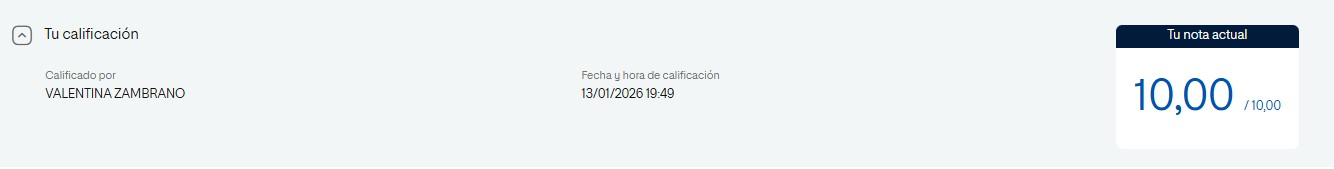
\includegraphics[width=1 \textwidth]{nota.jpg}
\end{figure}




\end{document}